%!TEX root = PhD_Thesis.tex
% Change page number to arabic numbers
\chapter{Introduction}
The interdisciplinary field of medical robotics aims to use robotic technology to improve the practice of medicine. Embodiments of this concept vary wildly, from telemanipulation systems that reduce the invasiveness of abdominal surgery, to exoskeletons that support patients in rehabilitation, to image-guided systems for bone resurfacing. Throughout medical robotics, a common theme is weighing the potential advantages of robotic technology, particularly in terms of patient outcome, against the added costs. Robots have many relevant advantages. Robots are precise and untiring. They can be made highly dexterous, and can operate in positions or environments that are unsafe for human clinicians. Robots also have many limitations. They are generally expensive. They require specialized infrastructure for installation and support. Like any electromechanical device, they will occasionally fail as a result of wear or damage, and this can have catastrophic effects in some clinical environments. 

This dissertation relates to the clinical specialty of interventional radiology, specifically to percutaneous (through needle-puncture of the skin) treatment of liver tumors. At a high level, the goal was to develop new technologies that would allow more patients to be treated with a percutaneous approach, rather than an invasive surgical intervention. This dissertation leverages prior work in robotic needle steering, a medical robotics research area which is described in the next section. 

\pagestyle{headings}
\setcounter{page}{1} 
\renewcommand{\thepage}{\arabic{page}}% Arabic page numbers

%%%%%%%%%%%%%%%%%%%%%%%%%%%%%%%%%%%%%%%%%%%%%%%%%%%%%%%%%%%%%%%%%%%%%%%%%%%%%%%%%%%%%%%%%%%%%%%%%%%%======================================================================
\section{Motivation}
%======================================================================
%%%%%%%%%%%%%%%%%%%%%%%%%%%%%%%%%%%%%%%%%%%%%%%%%%%%%%%%%%%%%%%%%%%%%%%%%%%%%%%%%%%%%%%%%%%%%%%%%%%
This section provides a clinical motivation for the dissertation. We begin with a brief overview of liver anatomy and liver cancer. We then discuss existing treatment options. Finally, the potential benefits of applying robotic needle steering in this application are outlined.

\begin{figure}[!t]
\centering
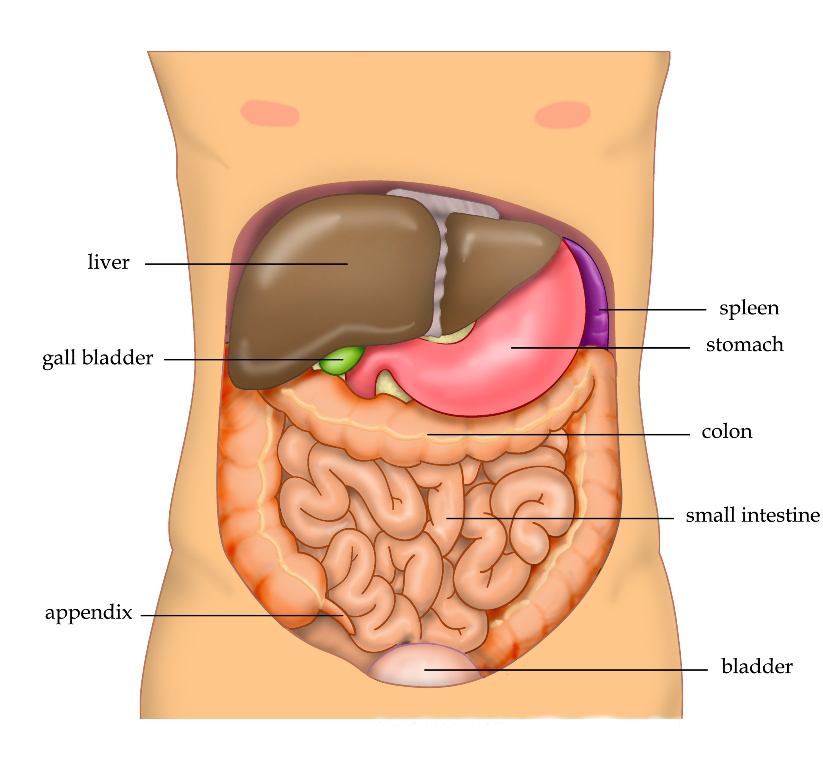
\includegraphics[width = 0.75\columnwidth]{./Images/Chapter1/liverIllustration.jpg}%
\caption[The human liver]{The human liver. Illustration by Ties van Brussel; tiesworks.nl (opensource).}
\label{fig:Ch1LiverAnatomy}
\end{figure} 

\subsection{Liver Cancer}
The liver is a glandular organ that sits in the right side of the abdomen in humans. It weighs approximately 1.2~kg to 1.5~kg, and is approximately 14~cm long on average in adults~\cite{Wolf1990,Kratzer2003}. The liver's primary function is to filter blood coming from the digestive tract before it passes on to the rest of the body. Structurally, the liver is divided into four lobes: the left, right, caudate, and quadrate lobes. Fig.~\ref{fig:Ch1LiverAnatomy} shows the left and right lobes, which are the largest. The liver is made up of very soft tissues called parenchyma, surrounded and supported by a tough capsule. Many vessels run through the liver, and it receives blood through two circulatory routes. The liver receives nutrient-rich, oxygen-poor blood from the spleen, pancreas and intestines through the hepatic portal vein. The liver also receives oxygen-rich blood through the hepatic artery. Blood from the two supplies mixes as it passes through the liver lobules---the basic functional units of the liver parenchyma---and into the hepatic veins. The blood then passes through the inferior vena cava to the heart.
   
Cancer is a disease caused by an uncontrolled division of abnormal cells. Liver cancer is a significant health concern in the United States. Liver cancer can be subdivided into primary liver cancer, where the disease originates in the cells of the liver, and secondary liver cancer, where the cancer originates in other organs and metastasizes to the liver. Approximately 35,660 new cases of primary liver cancer will be diagnosed in the United States in 2015, and approximately 24,550 people will die of these cancers~\cite{AmericanCancer2015}. Secondary liver cancers occur more frequently. Common types of cancer such as breast, lung, and colon all metastasize to the liver. For example, a quarter of the approximately 130,000 patients diagnosed with colorectal cancer each year in the United States will develop liver metastases~\cite{Ananthakrishnan2006,CDC2015,Haddad2011}. Liver cancer is an even more significant health concern in other parts of the world. Liver cancer is the most common type of cancer in many countries in sub-Saharan Africa and Southeast Asia. More than 700,000 people are diagnosed with this cancer each year throughout the world, with more than 600,000 deaths annually~\cite{AmericanCancer2015}.

\begin{figure}[!t]
\centering
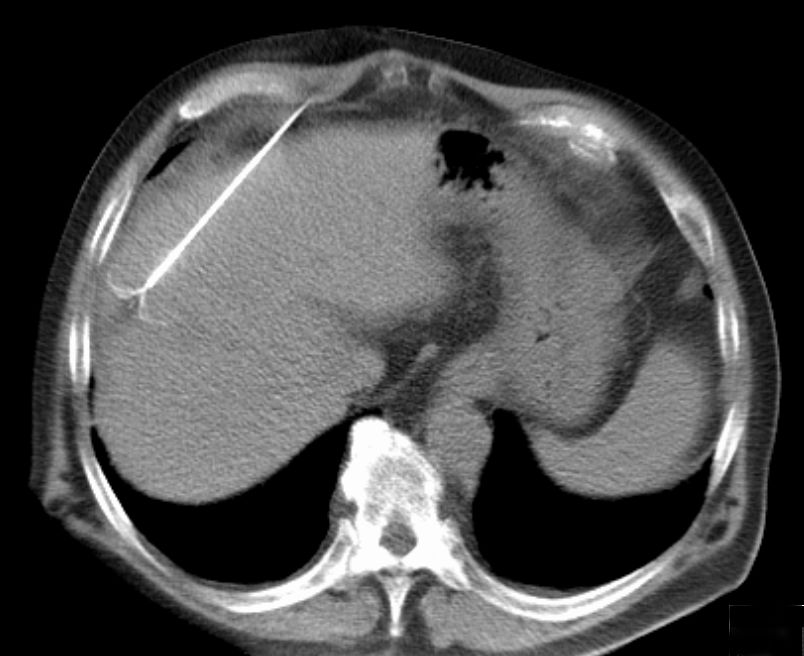
\includegraphics[width = 0.7\columnwidth]{./Images/Chapter1/liverAblation.jpg}%
\caption[Percutaneous radiofrequency ablation of a liver tumor]{Percutaneous radiofrequency ablation of a liver tumor, depicted in a CT image. The ablation needle enters at the top of the image and runs to the left. Electrodes extend from the rigid needle, and are used to ablate the tissue. Illustration by Hellerhoff (CC BY-SA 3.0).}
\label{fig:Ch1LiverAblation}
\end{figure}   

\subsection{Treatment of Liver Tumors}
Surgery, either for resection of the tumor or a liver transplant, is the only curative treatment of liver cancer, and offers the best long-term survival in select patients. However, approximately three quarters of patients are ineligible for surgery due to tumor size, type, or location; inadequate liver reserve; or other comorbidities. Percutaneous radiofrequency ablation (RFA) is a common, less invasive treatment option for liver cancer patients who are not eligible for resection or transplantation. In this procedure, long electrodes are inserted through the skin into the liver, and are used to ablate the cancer by depositing a high-frequency alternating current into the tissue. Fig.~\ref{fig:Ch1LiverAblation} shows a computed tomography (CT) image of this procedure. Microwave ablation is an alternative, relatively new percutaneous ablation technology which kills tissue through dielectric heating in an alternating electromagnetic field. Ethanol ablation is another alternative ablation technology for smaller, well-contained tumors, in which concentrated alcohol is injected into the tumor to kill the cancerous tissue. Although our focus in this thesis is on RFA of liver tumors, the techniques described relate equally well to microwave or ethanol ablation. 

Current techniques for percutaneous ablation of liver cancer suffer from significant limitations~\cite{Gervais2009}. Straight electrodes are unable to reach tumors in some portions of the liver because they are blocked by vasculature, lung, or other sensitive structures. Large tumors require multiple electrode insertions, with each puncture through the liver capsule increasing the risk of hemorrhage. This increased risk can make patients with advanced liver disease or severe comorbidities ineligible for the procedure. Successful treatment requires a margin of cancer-free tissue to be ablated around the tumor, in order to reduce the likelihood of recurrence~\cite{Kim2006}. For medium to large tumors, developing a sufficient ablative margin is highly dependent on the clinician's ability to locate the electrode tip over multiple passes using medical imaging (typically ultrasound or radiographic imaging) for guidance~\cite{Dodd2001}. 
 
\subsection{Robotic Needle Steering}
Robotic needle steering enables the insertion of flexible needles along controlled, curved, three-dimensional (3D) paths through tissue~\cite{DiMaio2005,Webster2006}. Robotic needle steering offers the potential to improve percutaneous ablation of liver tumors in several ways. Specifically, robotic needle steering may allow clinicians to (1) correct for errors during insertion and reach a target position with superior accuracy compared to manual insertion, (2) steer around obstacles to previously unreachable targets, and (3) reach multiple targets from a single insertion site, thus reducing the risk of complications such as hemorrhage or infection.

%%%%%%%%%%%%%%%%%%%%%%%%%%%%%%%%%%%%%%%%%%%%%%%%%%%%%%%%%%%%%%%%%%%%%%%%%%%%%%%%%%%%%%%%%%%%%%%%%%%%======================================================================
\section{Prior Work}
%======================================================================
%%%%%%%%%%%%%%%%%%%%%%%%%%%%%%%%%%%%%%%%%%%%%%%%%%%%%%%%%%%%%%%%%%%%%%%%%%%%%%%%%%%%%%%%%%%%%%%%%%%
This section provides a review of relevant existing research. We begin by describing methods for robotic needle steering; that is, using a robotic system to steer a flexible needle through tissue. Next we review existing methods for automatic segmentation of needles from ultrasound image data, as one of the main focuses of the dissertation is using ultrasound imaging for control of a needle steering robot. Control algorithms for needle steering robots are also discussed. Finally, the state of robotic needle steering research is discussed, in order to better situate the dissertation.

\subsection{Techniques for Needle Steering}
A number of methods have been described for steering needles through tissue. A recent review is given in~\cite{vandeBerg2014}. DiMaio and Salcudean~\cite{DiMaio2005} and Glozman and Shoham~\cite{Glozman2007} used lateral robotic manipulation of the needle base during insertion to steer the needle. Mallapragada et al.~\cite{Mallapragada2009} and Torabi et al.~\cite{Torabi2009} used robotic manipulation of artificial tissues around a needle during insertion to steer the needle. Okazawa et al.~\cite{Okazawa2005} used a precurved stylet that could be rotated and translated relative to a straight needle shaft to steer a manually inserted needle device. The same concept of overlapping pre-curved sections has been applied in multiple stages in the active cannula robots described by Sears and Dupont~\cite{Sears2006} and Webster et al.~\cite{Webster2009}. Kratchman et al.~\cite{Kratchman2011} described tendon actuation systems designed to steer flexible needle shafts in solid tissue. Ayvali et al.~\cite{Ayvali2012}, Datla et al.~\cite{Datla2014}, and Ryu et al.~\cite{Ryu2014} have used shape memory alloy (SMA) actuators to articulate needle sections, with the latter system using optically actuated SMA tendons to allow compatibility with MRI systems. Ko and Rodriguez y Baena~\cite{Ko2013} have described a biologically inspired needle that steers by adjusting the relative offset between parallel sections. Our work focuses on bent-tip steerable needles: flexible needle shafts with bent distal sections. 

Bent-tip needles naturally steer along curved paths during insertion as a result of the net lateral force acting at the distal end of the needles~\cite{Webster2006}. A duty-cycle control approach, first proposed by Minhas et al.~\cite{Minhas2007}, allows curvature to be varied by alternating periods of needle rotation. A bent-tip needle with a passive flexure was introduced by Swaney et al.~\cite{Swaney2013} to reduce tissue damage caused by the bent tip during rotation. Similar flexible needles with bevel tips~\cite{OLeary2003,Alterovitz2005} and curved distal sections~\cite{Wedlick2009} have also been described. A tendon-actuated bent-tip steerable needle was described by van de Berg et al.~\cite{vandeBerg2015}. This design incorporates a two degree-of-freedom ball and socket joint with a conical tip to achieve 3D steering.

\subsection{Automatic Segmentation of Needles from Ultrasound}
A large amount of prior art exists on the automatic segmentation of needles from B-mode (grayscale) ultrasound data, with much of it focused on segmenting straight needles using a variant of the Hough transform. Although the Hough transform is computationally intensive, real-time segmentation of straight needles has been demonstrated using variations on the algorithm, including dual-plane projections~\cite{Ding2003b}, coarse-fine sampling~\cite{Ding2003a,Zhou2008}, and parallel implementation on a graphics processing unit~\cite{Novotny2007}. Other similar algorithms, such as the parallel integral projection transform, have also been applied~\cite{Barva2008}. Similar methods have been described for segmenting curved needles. Slightly curved needles can be segmented using a standard Hough transform method~\cite{Okazawa2006,Aboofazeli2009}, while more strongly curved needles can be segmented by including a parametrization of needle bending~\cite{Neshat2008,Okazawa2006,Uhercik2010}.

\subsection{Doppler-Based Segmentation}
\label{sec:Doppler-BasedSegmentation}
Ultrasound Doppler is a diagnostic technique that measures frequency shifts in reflected ultrasonic waves that result from motion. Color and power Doppler imaging, which are available on most modern ultrasound systems, are commonly applied to overlay blood flow data on B-mode ultrasound. Vibrating solid objects have also been shown to produce recognizable Doppler signals~\cite{Holen1985}. This concept has been applied to localize straight needles~\cite{Armstrong2001,Feld1997,Hamper1991} and needle tips~\cite{Harmat2006} in 2D ultrasound, as well as instruments in cardiac interventions~\cite{Fronheiser2008,Reddy2008} and other applications~\cite{McAleavey2003,Rogers2009}. This technique has not previously been applied to segment highly curved needles.

\subsection{Control Approaches for Robotic Needle Steering}
There is significant prior art relevant to image-guided control of needle steering, both for bent-tip steerable needles and other approaches. DiMaio and Salcudean formulated rigid needle insertion as a trajectory planning and control problem, defining a needle manipulation Jacobian for base control~\cite{DiMaio2005}. Glozman and Shoham~\cite{Glozman2007} and Neubach and Shoham~\cite{Neubach2010} used inverse kinematics to control base-manipulation needle steering, with X-ray and ultrasound image feedback respectively. Ko and Rodriguez y Baena used a model-predictive control algorithm for trajectory-following control of a bio-inspired actuated flexible needle~\cite{Ko2012}. For bent-tip steering, a number of control approaches have been described based on a nonholonomic model of steerable needle motion in tissue~\cite{Webster2006}. Reed et al. demonstrated image-guided needle steering in a planar workspace~\cite{Reed2011}, by combining a planar motion planner~\cite{Alterovitz2008}, an image-guided controller~\cite{Kallem2009}, and a torsion compensator~\cite{Reed2009}. Wood et al. formulated trajectory tracking controllers based on duty cycling for 2D~\cite{Wood2010} and 3D~\cite{Wood2013} trajectories. Bernardes et al.\ combined closed-loop image feedback with intraoperative replanning to deal with obstacles and dynamic workspaces~\cite{Bernardes2013}. Rucker et al.~\cite{Rucker2013} used a sliding mode controller with feedback from an electromagnetic tracking system. This control scheme has the advantage that it does not require any prior knowledge of needle curvature. Abayazid et al. demonstrated bent-tip needle control in gelatin and chicken breast using a robotically controlled ultrasound transducer to track the tip~\cite{Abayazid2014}. The steerable needle described by van de Berg et al.~\cite{vandeBerg2015} uses an integrated fiber Bragg grating (FBG) shape sensor and proportional-integral control of the tendon-actuated tip. 

Several schemes for teleoperation or human-in-the-loop control of steerable needles have been proposed. Romano et al. implemented several joint-space control schemes, comparing autonomous, manual, and combined control of the insertion and rotation of the steerable needle~\cite{Romano2007}. Majewicz and Okamura implemented task-space teleoperation using a 3D display and a haptic device as a master input~\cite{Majewicz2013}. In a human user study, they found task-space teleoperation resulted in lower time to target and insertion length than joint-space teleoperation. Pacchierotti et al. implemented a teleoperation system that combined kinesthetic and
vibratory feedback to provide information about ideal insertion and rotation of the steerable needle~\cite{Pacchierotti2014}.

\subsection{Current State of Needle Steering Research}
Robotic needle steering has existed solely as a research concept for over a decade. The work on rigid needle steering by DiMaio and Salcudean in 2005~\cite{DiMaio2005} appears to be the first in this area. At roughly the same time, Webster et al. suggested using flexible needles with asymmetric tips to steer through solid organs~\cite{Webster2005}. Since then there have been dozens of journal and conference articles on this topic, all motivated by the potential benefits of achieving controlled, curved needle paths through tissue. Interestingly for a medical robotics topic, there has been almost no progression towards clinical or patient studies. Steerable needles have only been applied in one \textit{in vivo} test~\cite{Majewicz2012}, which measured open-loop steerable needle curvature in different tissues, without simulating a clinical scenario or performing closed-loop targeting.

To date, needle steering research has been largely the domain of roboticists. Experimental validation of many of the methods described above has been limited to artificial tissues. These artificial tissues provide only limited validation, as their mechanical properties are significantly different from biological tissues~\cite{Wedlick2012}. Without methods for medical image feedback, many needle steering experiments have been constrained to 2D workspaces in transparent artificial tissues such as agar or PVC rubber, with optical cameras used to simulate medical imaging. Although some studies have applied more realistic medical imaging methods~\cite{Glozman2007,Neubach2010,Abayazid2014}, they have generally been evaluated in tightly controlled bench-top settings, yielding best-case needle visibility.

The research described in this dissertation was intended to move robotic needle steering closer to the clinical domain, by targeting a specific percutaneous intervention (ablation of liver tumors), and solving several of the largest technical problems specific to that procedure. In particular, we focused on real-time medical imaging of the needle, an estimation scheme for tracking the pose of the steerable needle tip, and a complete system for human-in-the-loop control. We also developed new methods to allow bent-tip steerable needles to achieve tighter curvature in liver tissue. In all these areas, our focus was on clinically realistic implementations that were validated in biological tissues.  

%%%%%%%%%%%%%%%%%%%%%%%%%%%%%%%%%%%%%%%%%%%%%%%%%%%%%%%%%%%%%%%%%%%%%%%%%%%%%%%%%%%%%%%%%%%%%%%%%%%%======================================================================
\section{Contributions}
%======================================================================
%%%%%%%%%%%%%%%%%%%%%%%%%%%%%%%%%%%%%%%%%%%%%%%%%%%%%%%%%%%%%%%%%%%%%%%%%%%%%%%%%%%%%%%%%%%%%%%%%%%
The major contributions of the research described in this dissertation can be summarized as follows:
\begin{itemize}
\item Proposed and validated a method for automatic segmentation of a steerable needle from 3D ultrasound data, based on applying mechanical vibration to the steerable needle in order to make it visible in power Doppler ultrasound.
\item Proposed and validated an estimation scheme based on an unscented Kalman filter that allows infrequent, noisy medical image measurements (e.g., from the Doppler segmentation) to be used to track the pose of the steerable needle tip.
\item Implemented and validated a system for freehand-3D-ultrasound-guided needle steering, which combines the output of the unscented Kalman filter with existing needle steering control algorithms, to allow a clinician to manually visualize target anatomy while simultaneously providing image feedback for automatic control.  
\item Completed a workspace analysis of percutaneous RFA of liver tumors, using medical image analysis to set a procedure-specific requirement for steerable needle curvature.  
\item Performed finite-element modeling and experimental studies to demonstrate that the required steerable needle curvature can be achieved in liver tissue through optimization of tip geometry. Motivated by these results, proposed and validated an articulated-tip steerable needle mechanism.   
\end{itemize}

%%%%%%%%%%%%%%%%%%%%%%%%%%%%%%%%%%%%%%%%%%%%%%%%%%%%%%%%%%%%%%%%%%%%%%%%%%%%%%%%%%%%%%%%%%%%%%%%%%%%======================================================================
\section{Dissertation Overview}
%======================================================================
%%%%%%%%%%%%%%%%%%%%%%%%%%%%%%%%%%%%%%%%%%%%%%%%%%%%%%%%%%%%%%%%%%%%%%%%%%%%%%%%%%%%%%%%%%%%%%%%%%%
This dissertation is composed of six chapters. This introductory chapter has provided the clinical motivation for the work, a survey of relevant research literature, and a summary of the contributions of the dissertation. Chapter 2 describes methods for real-time automatic segmentation of a steerable needle from 3D ultrasound data, as well as a general closed-loop control framework which will be applied throughout the dissertation. Chapter 3 describes a workspace analysis of percutaneous RFA of liver tumors, as well as finite-element modeling, experimental studies and mechanism design intended to achieve improved steerable needle curvature in liver tissue. Chapter 4 describes a new estimation scheme based on an unscented Kalman filter, which is used to track the pose of the steerable needle tip using the noisy ultrasound segmentation results, in order to enable closed-loop steering. Chapter 5 describes methods for human-in-the-loop control of needle steering using freehand 3D ultrasound imaging. This approach is validated in a clinical experiment, steering towards simulated targets in a porcine cadaver. Finally, Chapter 6 summarizes the results of the research, reviews the contributions made in this dissertation, and provides suggestions for future work.